\documentclass[10pt,a4paper]{article}
\usepackage[margin=2.2cm]{geometry}
\usepackage{fontspec}
\usepackage{kotex}
\setmainfont{Apple SD Gothic Neo}
\setsansfont{Apple SD Gothic Neo}
\usepackage{amsmath,amssymb}
\usepackage{graphicx}
\usepackage{booktabs}
\usepackage{caption}
\usepackage[dvipsnames]{xcolor}
\usepackage[colorlinks=true,linkcolor=MidnightBlue,citecolor=MidnightBlue,
            urlcolor=MidnightBlue]{hyperref}
\usepackage{titlesec}
\titleformat{\section}{\large\bfseries}{\thesection}{0.6em}{}
\captionsetup{font=small,labelfont=bf}
\setlength{\parskip}{0.35em}
\setlength{\parindent}{0pt}

\usepackage{mdframed}
\newmdenv[linewidth=0.4pt,linecolor=gray!60,backgroundcolor=gray!5,
          innertopmargin=6pt,innerbottommargin=6pt,skipabove=8pt,skipbelow=8pt]{claimbox}
\newcommand{\claim}[2]{\begin{claimbox}\textbf{주장.} #1\par\smallskip
  \textcolor{gray!70}{\textbf{반증 조건.} #2}\end{claimbox}}

\title{\bfseries 관객과 조회가 같은 모양으로 식는다\\[2pt]
\large 문패 재개 $1$탄 --- 영화 실측 곡선이 위키 무리와 겹쳤다}
\author{월드모델 실험실 · 노트 $838$}
\date{2026-08-08}
\begin{document}\maketitle

\section{한 줄}

$813/814$ 가 문패로 걸어 둔 물음 --- \emph{``진폭 큰 안정 도메인이 오면 형태
공유의 판정력이 서나''} --- 를 드디어 실측 곡선으로 쟀다. 영화 학습 곡선
$161$편(관측 $\geq 60$일 · 자기 바닥 $0.0395$ --- 기존 무리보다 안정 · 진폭
$6.76$ --- 판 최대 확정): \textbf{영화-모바일 같다 $0.95\times$(바닥 아래) ·
게임 $1.64\times$ · 세계애니 $2.38\times$ 모른다 --- `다르다' $0$.} $7$일 평활
팔도 같은 그림이라 \textbf{주간 진동은 차이의 원천이 아니다.} 갈래 $3$: 무리
확장 후보.

\begin{figure}[t]\centering
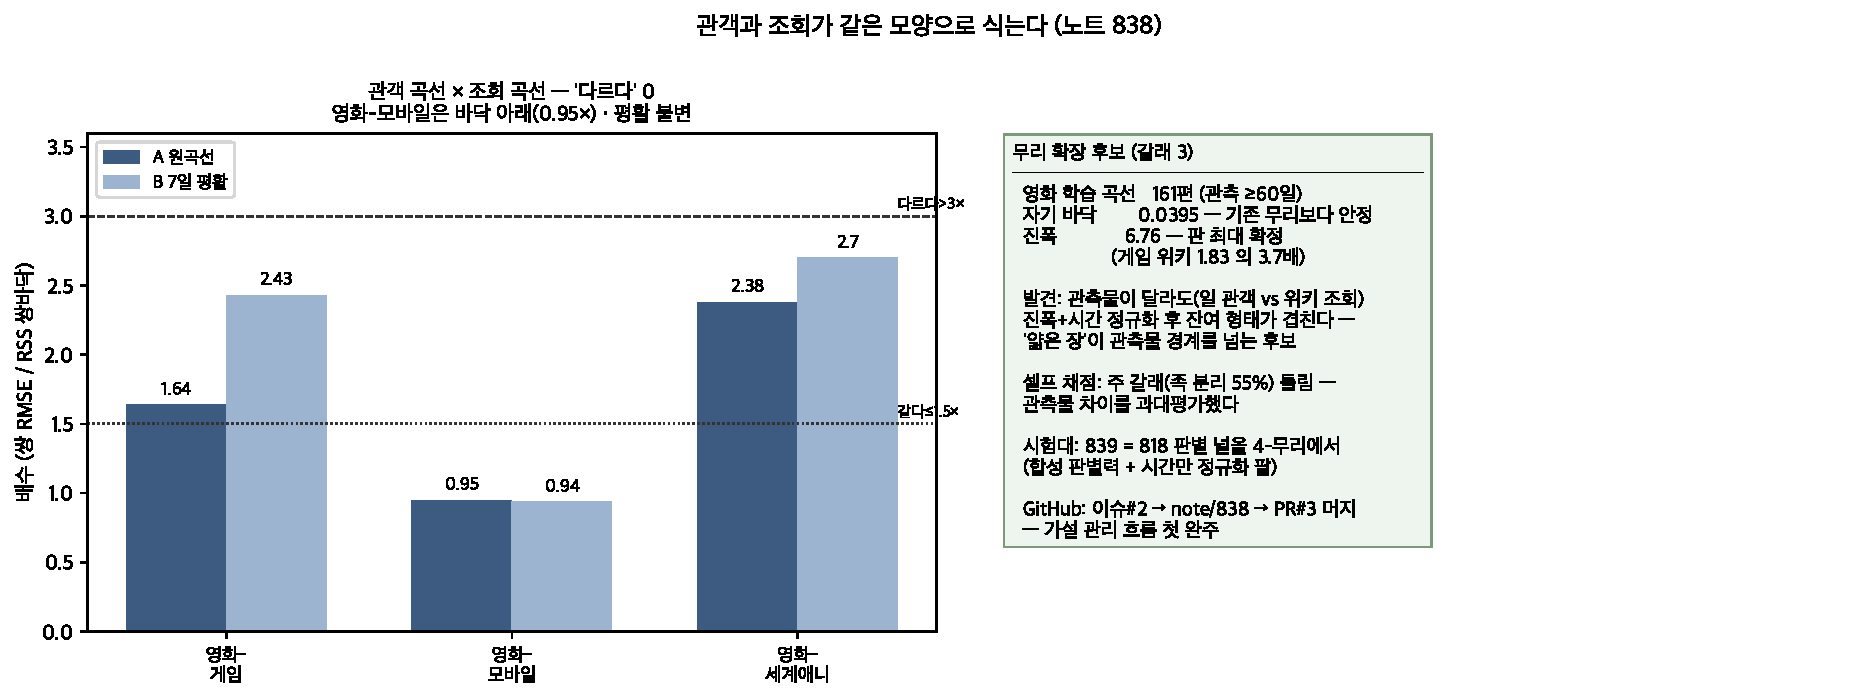
\includegraphics[width=0.97\textwidth]{figs/cool.pdf}
\caption{왼쪽: 두 팔의 배수. 오른쪽: 요약과 시험대.}
\end{figure}

\section{관측물 경계를 넘는 얇은 장}

\claim{\textbf{일 관객 수와 위키 조회 수는 다른 물리량인데, 진폭$+$시간 정규화
후 잔여 형태가 겹친다.} 내 주 예측(족 분리 $55\%$ --- 관측물이 다르니 다를
것)은 틀렸고, 그 틀림이 발견이다: $818$ 의 `얇은 장'이 매체 경계(만화 $\to$
애니)만이 아니라 \textbf{관측물 경계(주의 $\to$ 소비)까지 넘는 후보}가 됐다.
안정 무리는 $3 \to 4$(게임 · 모바일 · 세계애니 · 영화) 확장 후보.}
{$814/818$ 의 교훈 그대로 --- `같다'는 두 자유도 제거 후의 약한 결과다.
시험대는 $839$: $818$ 의 판별 널(합성 판별력 $+$ 시간만 정규화 팔)을
$4$-무리에서, 이번엔 실측 영화 곡선을 넣고 재실행한다. 부 예측 채점: 진폭
최대($90\%$) 적중 · `원곡선 전부 다르다'($75\%$) 크게 틀림. GitHub 가설
관리(이슈 \#$2$ $\to$ PR \#$3$ 머지)가 이 노트로 첫 완주. 판 $\rho$
$0.4710$ 그대로.}

\end{document}
